
\documentclass[ms.tex]{subfiles} 
\begin{document} 

\section{Results} 
\label{sec:results} 

\begin{figure*} 
\centering 
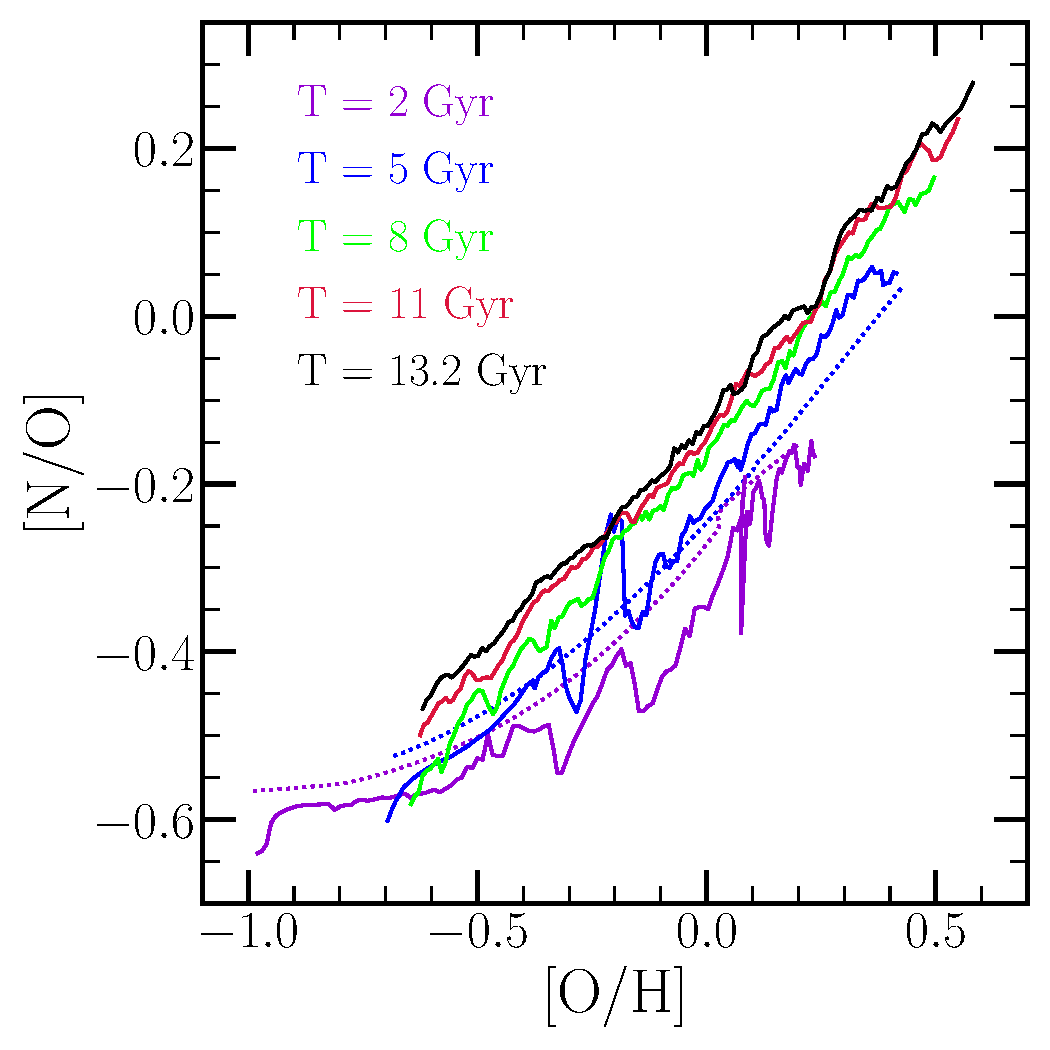
\includegraphics[scale = 0.45]{no_oh_timeevol.pdf} 
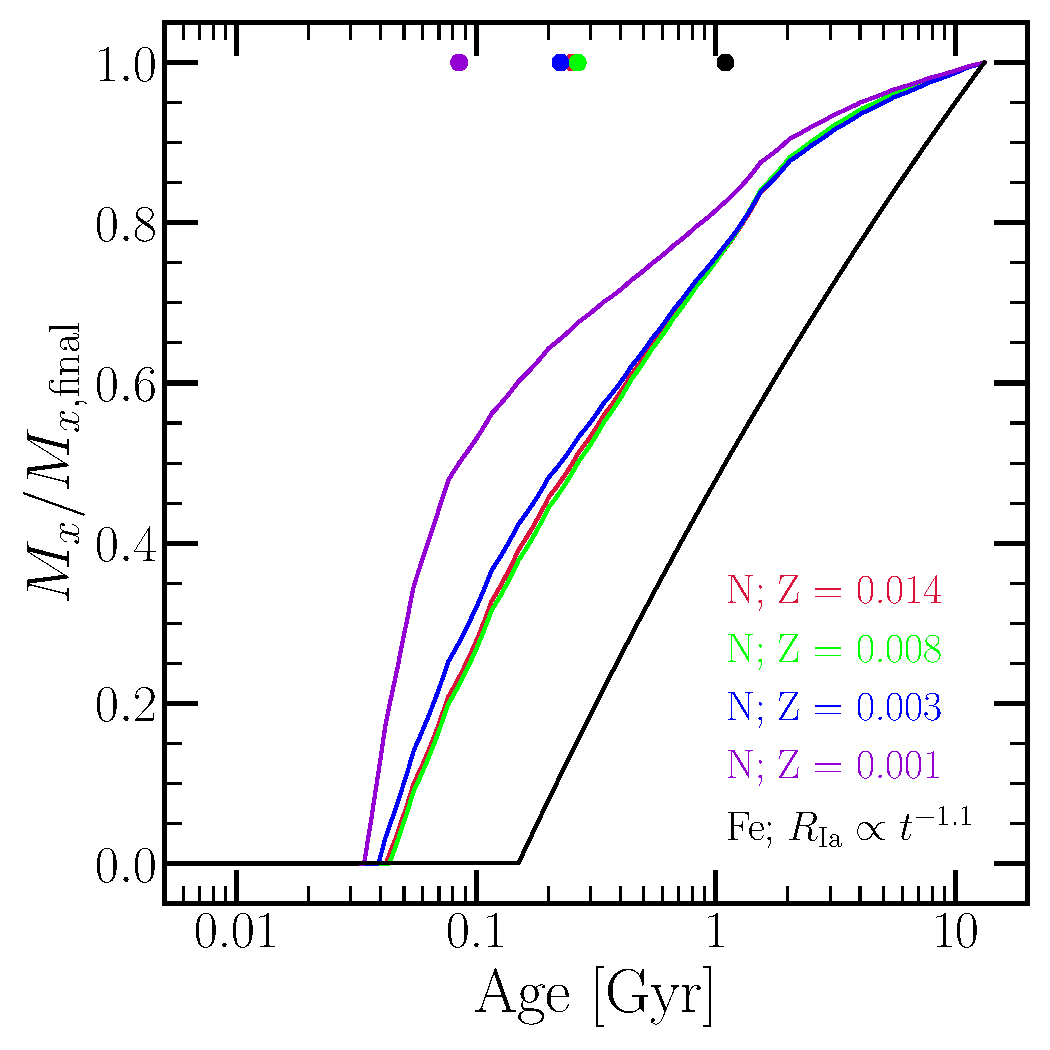
\includegraphics[scale = 0.45]{ssp_production.pdf} 
\caption{
\textbf{Left}: The time evolution of the gas-phase [N/O]-[O/H] relation in 
our fiducial model with the~\cristallo~yields (solid colored lines). 
Dotted lines denote the resulting relation when stellar migration is 
neglected at~$T$ = 2 and 5 Gyr. 
\textbf{Right}: The net mass of N produced by AGB stars from a single stellar 
population assuming four initial metallicities and the~\cristallo~yields 
(colored lines). 
The black line denotes the same for Fe assuming the~$t^{-1.1}$ power-law delay 
time distribution adopted in our models. 
All values are normalized to the total mass produced at an age of 13.2 Gyr. 
Points at the top of the panel denote the ages at which 50\% of the total mass 
has been produced. 
} 
\label{fig:no_oh_timeevol_ssp} 
\end{figure*} 

\begin{figure*} 
\centering 
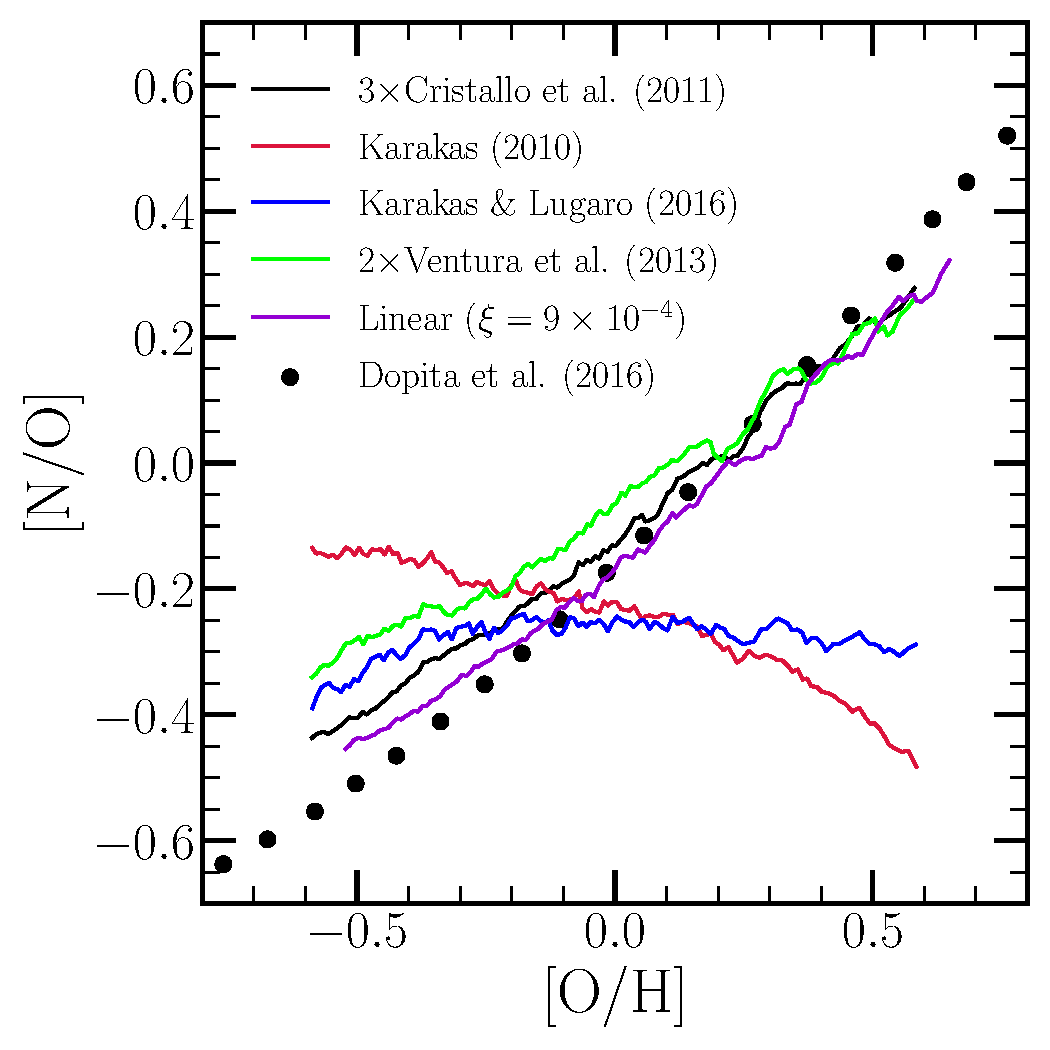
\includegraphics[scale = 0.45]{no_oh_predictions.pdf} 
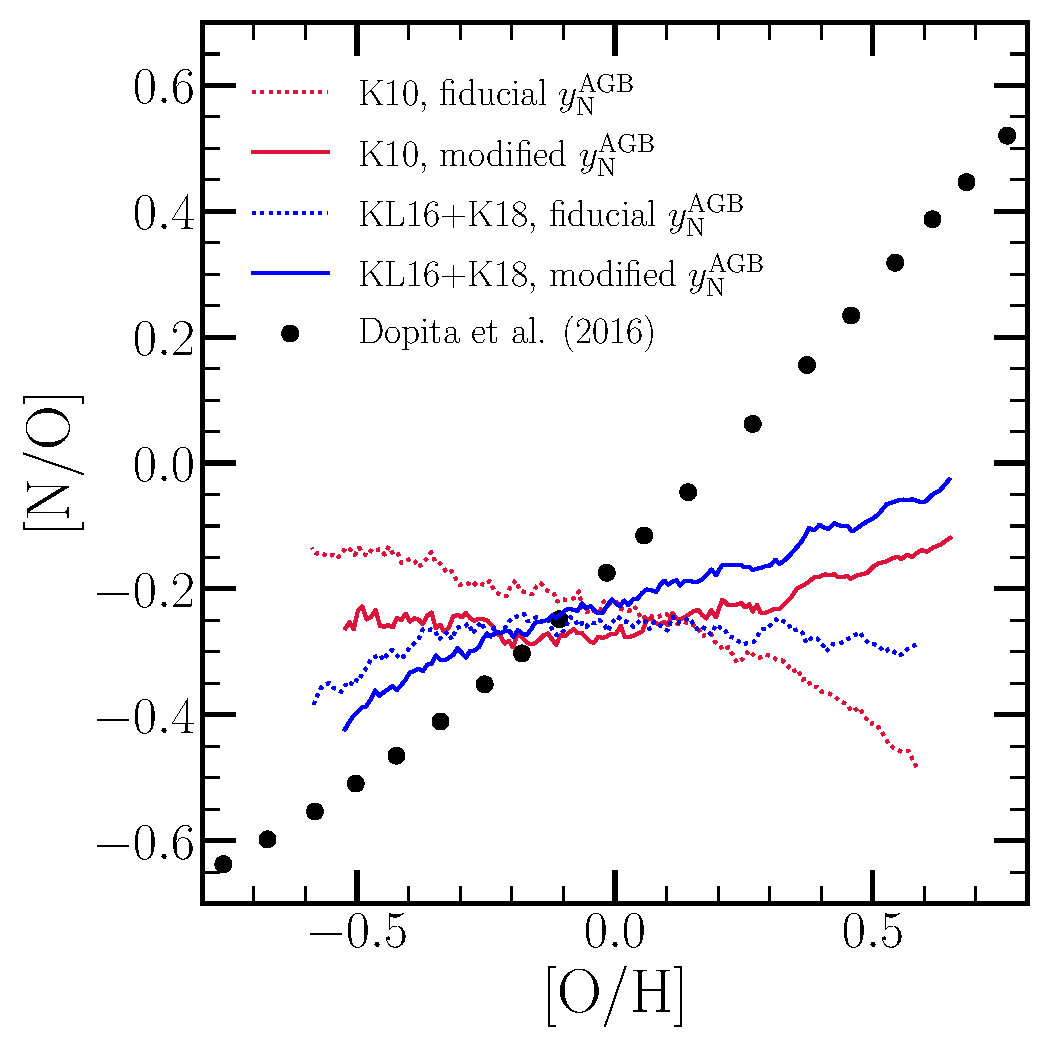
\includegraphics[scale = 0.45]{no_oh_predictions_karakas.pdf} 
\caption{
\textbf{Left}: The present day gas-phase [N/O]-[O/H] relation predicted by our 
fiducial model with each of the yield sets described 
in~\S~\ref{sec:methods:yields:agb}. 
For observational reference, we plot the population-averaged trend for local 
stars and HII regions reported by~\citet{Dopita2016}. 
\textbf{Right}: The same as the left-hand panel, but comparing the predictions 
made by the~\karakasten~and~\karakas~yields with our fiducial value 
of~$y_\text{N}^\text{CC}$ (dotted lines, same as left-hand panel) to those with 
the alternate forms of~$y_\text{N}^\text{CC}$ (solid lines) given by equation X 
for the~\karakasten~yields and equation Y for the~\karakas~yields. 
} 
\label{fig:no_oh_predictions} 
\end{figure*} 

\begin{figure*} 
\centering 
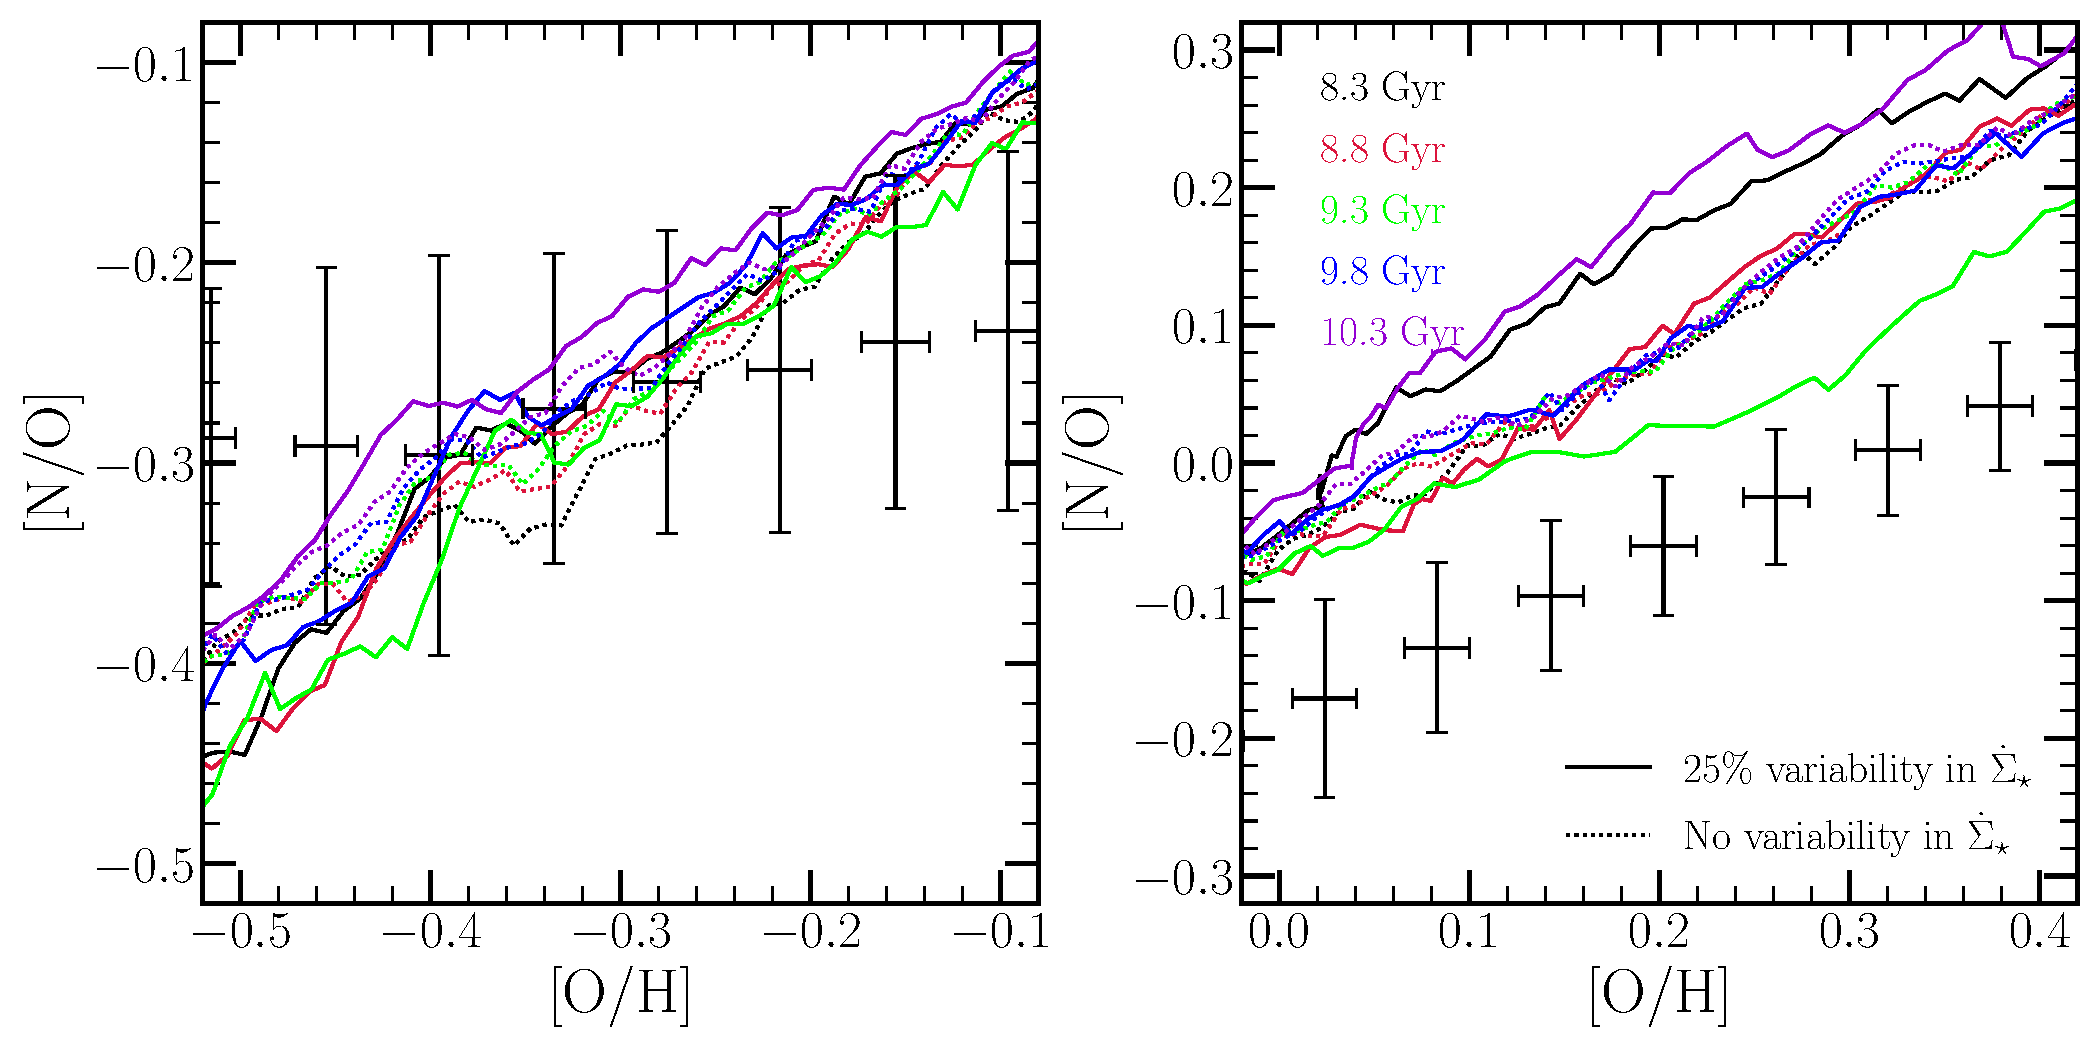
\includegraphics[scale = 0.45]{no_oh_modsfr.pdf} 
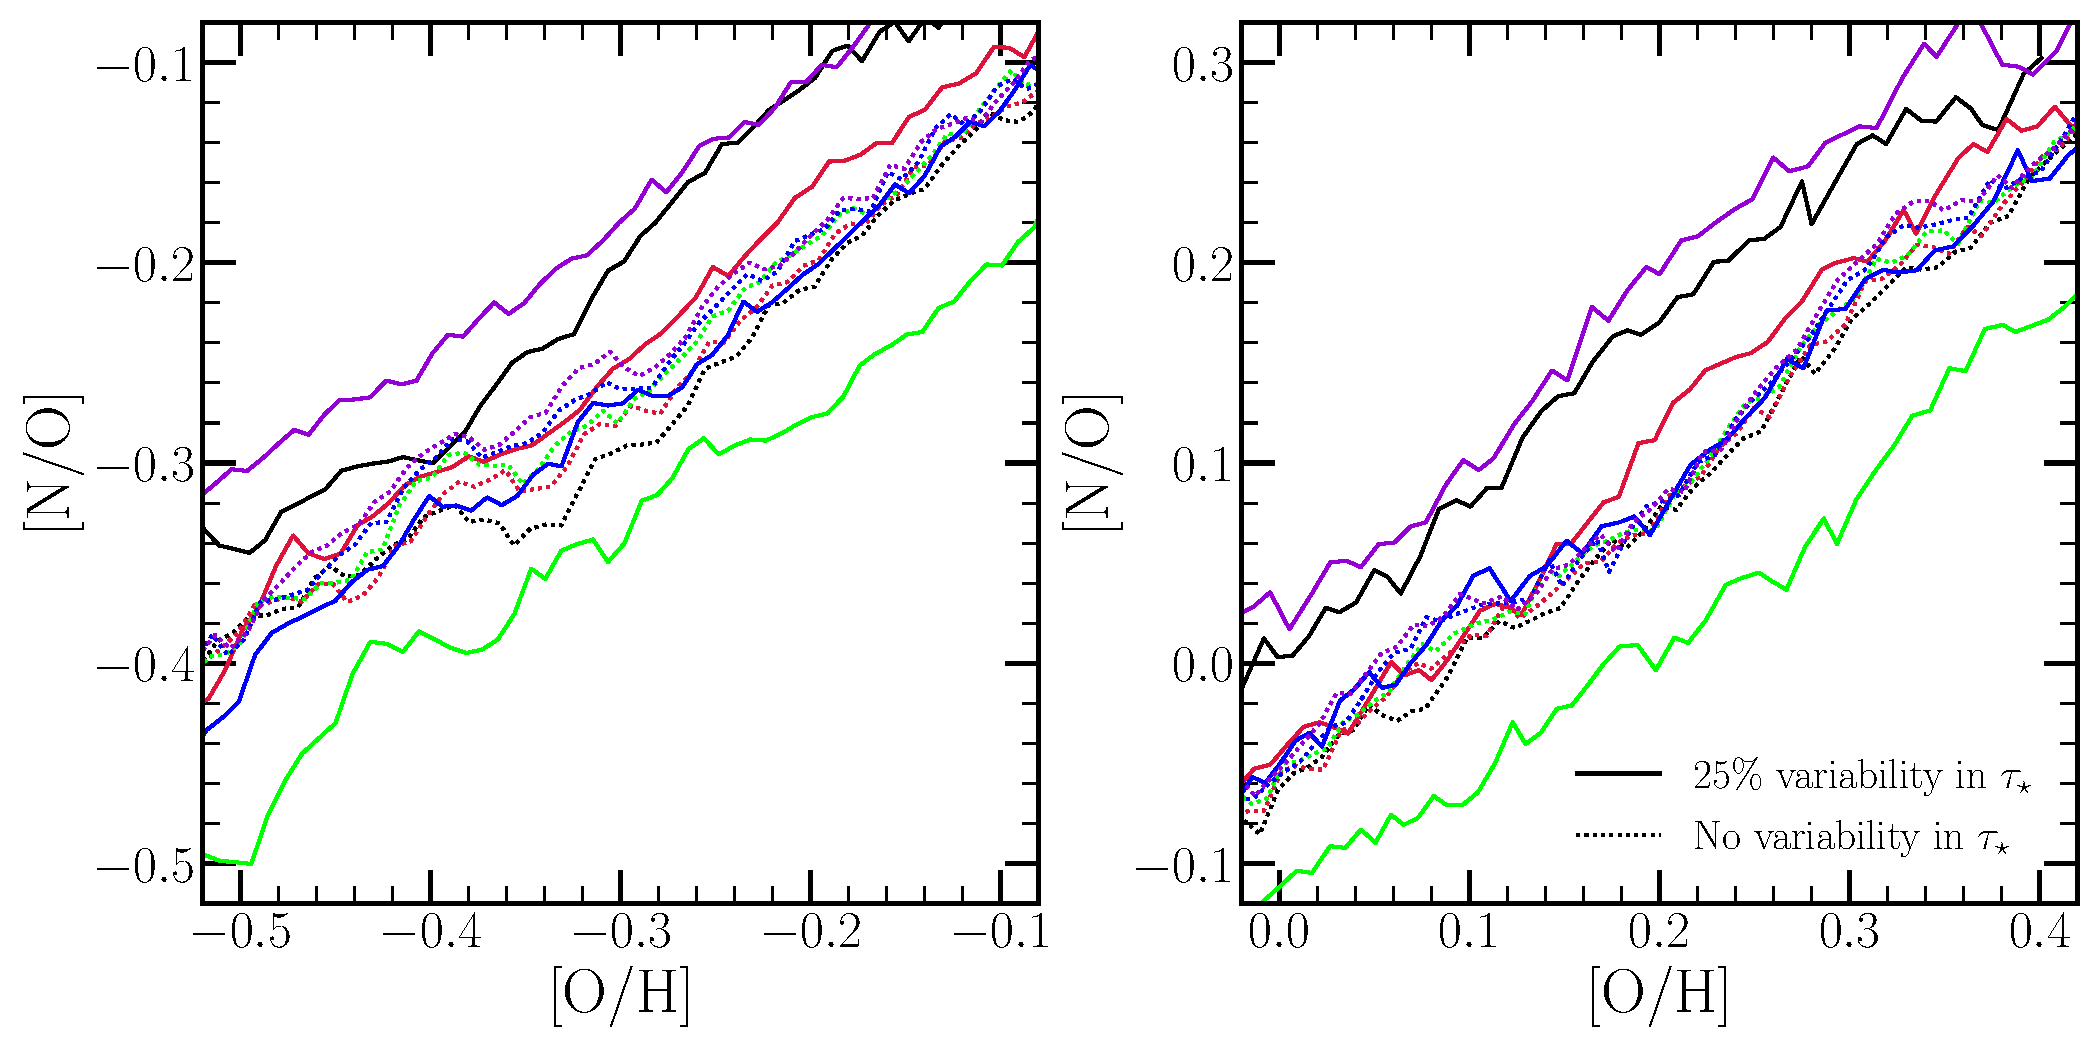
\includegraphics[scale = 0.45]{no_oh_modsfe.pdf} 
\caption{
One cycle of variability in the gas-phase [N/O]-[O/H] relation at low [O/H] 
(left) and high [O/H] (right) induced by 25\% sinusoidal variations in the SFR 
(top) and in the SFE (bottom). 
Solid lines denote the models with some source of variability, and dotted lines 
denote the fiducial model with no variability; all models take into account the 
effects of stellar migration. 
} 
\label{fig:no_oh_mods} 
\end{figure*} 

\end{document} 

